\subsection{Manejador de pedidos de nivel 5 + cliente}

\begin{figure}[H]
   \centering
   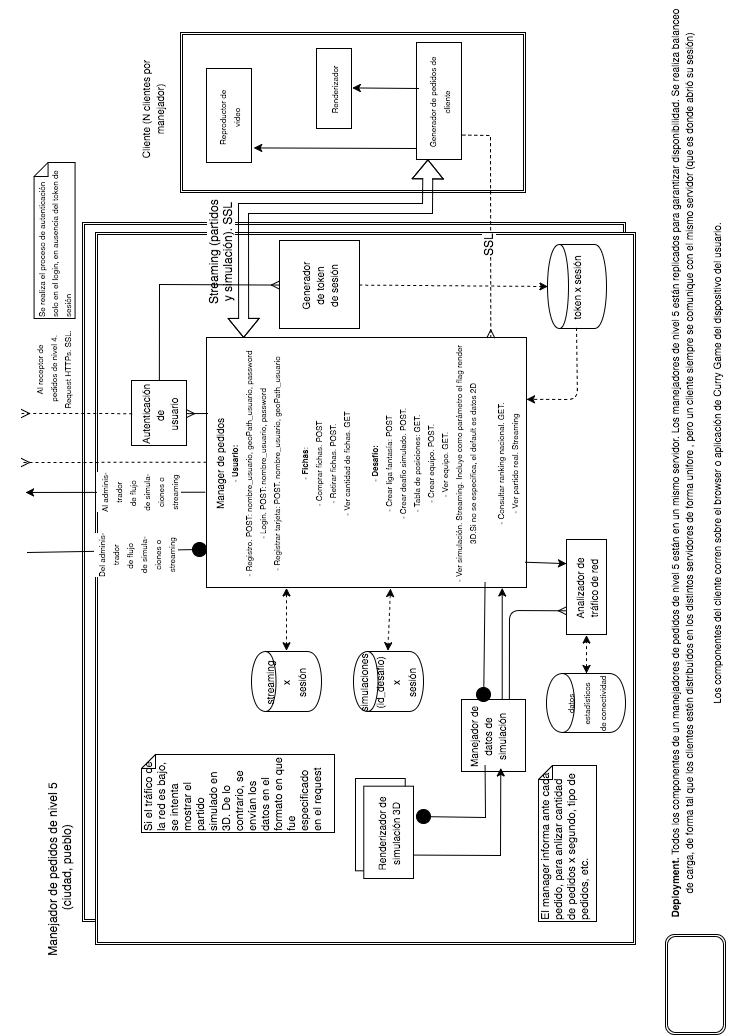
\includegraphics[height=0.95\textheight]{reentrega/imagenes/nivel-5-manejador-cliente.png}
   \caption{Manejador pedidos de nivel 5.}
\end{figure}

Toda interacción, salvo el registro, comienza con la creación de una sesión, que se utiliza tanto como mecanismo de seguridad como performance, para no autenticar al usuario por cada pedido que desea realizar.
Cada sesión está representada con un token, que se calcula durante el proceso de login.

El cliente envía usando SSL su usuario y contraseña. El manejador le forwardea el pedido al manejador de usuarios de nivel 4, y en el caso de que la autenticación sea exitosa se inicia una sesión representada por un token, que es almacenada en un repositorio. El token se envía encriptado al cliente, y en cada pedido que este haga deberá incluírlo. De esta manera, mientras la sesión no expire, el manager de pedidos verificará la existencia de una sesión abierta para dicho pedido lo cual ahorra un tiempo considerable.

Los usuarios pueden realizar distintos tipos de pedidos, enumerados en el manager de pedidos. La mayoría de ellos, con excepción del rendering de las simulaciones y el streaming de partidos se forwardean al receptor de pedidos del nivel 4.

Un pedido para ver una simulación se traduce en una suscripción al conector de 'Administrador de flujo de simulaciones', que a partir de ese momento comenzará a publicar el detalle de las simulaciones. Todas las sesiones que han solicitado ver la simulación de un determinado desafío se guardan en un repositorio. Con esto se logran 2 objetivos: Por un lado, evitar enviar suscripciones a simulaciones de desafíos de los que ya se está siendo notificado (Performance, Disponibilidad. No saturar la red). Por el otro, cuando llega un evento de la simulación de un desafío, saber qué sesiones están siguiendo dicho desafío para poder enviarles los datos.
El streaming de los partidos reales sigue un proceso análogo.

Ante cada pedido, el manager le informa al analizador de tráfico acerca de este nuevo pedido y su tipo (si es un login, consulta de ranking, pedio de streaming o simulación, etc).

Los pedidos de ver una simulación toman como parámetro el modo en que desea recibirse. Por default se asume que son datos en formato rendering de 2D (que son los que cualquier dispositivo puede reproducir). Sin embargo, un usuario puede indicar querer recibir datos de rendering 3D si su dispositivo lo soporta.

En el momento en que llegan datos de una simulación, el manejador de datos de simulación consulta al analizador acerca del estado de la red. En el caso en el que la misma no esté sobrecargada, es el mismo manejador de pedidos de nivel 5 quien renderiza en 3D los datos y los envía como video, con el objetivo de que la mayor cantidad de usuarios (sobre todo aquellos que no tienen un dispositivo poderoso para renderizar los datos 3D) puedan gozar de la simulación en su máxima calidad. Por el contrario, si la red está congestionada (por ejemplo, si muchos usuarios están viendo streaming de partidos reales o simulaciones) entonces se envían los datos sin procesar.
